\begin{frame}[fragile]{Sequence to Sequence (Seq2Seq)}

    \begin{itemize}
        \item Many NLP tasks viewed sequence-to-sequence:
              \begin{enumerate}
                  \item Summarization (whole document $\rightarrow$ shorter text)
                  \item Machine Translation (one language $\rightarrow$ target language)
              \end{enumerate}
    \end{itemize}
    \begin{center}
        \tikzset{arrow/.style={-stealth, thick, draw=gray!80!black}}
        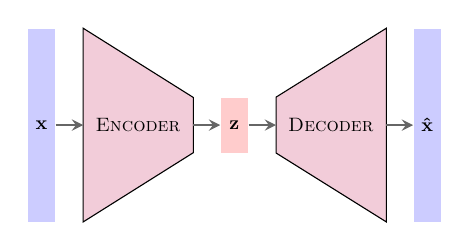
\begin{tikzpicture}[scale=0.7, every node/.style={scale=0.7}]
            \node[fill=blue!20, minimum width=0.5cm, minimum height=3.5cm] (X) at (0,0) {$\mathbf x$};
            \draw[fill=purple!20] ([xshift=0.5cm]X.north east) -- ([xshift=2.5cm,yshift=0.5cm]X.east) -- ([xshift=2.5cm,yshift=-0.5cm]X.east) -- ([xshift=0.5cm]X.south east) -- cycle;
            \node at (1.75,0) {\textsc{Encoder}};
            \node[fill=red!20, minimum width=0.5cm, minimum height=1.0cm] (Z) at (3.5cm,0) {$\mathbf z$};
            \draw[fill=purple!20] ([xshift=0.5cm]Z.north east) -- ([xshift=2.5cm,yshift=1.25cm]Z.north east) -- ([xshift=2.5cm,yshift=-1.25cm]Z.south east) -- ([xshift=0.5cm]Z.south east) -- cycle;
            \node at (5.25,0) {\textsc{Decoder}};
            \node[fill=blue!20, minimum width=0.5cm, minimum height=3.5cm] (Xp) at (7,0) {$\mathbf{\hat{x}}$};
            \draw[arrow] (X.east) -- ([xshift=0.5cm]X.east);
            \draw[arrow] ([xshift=-0.5cm]Z.west) -- (Z.west);
            \draw[arrow] (Z.east) -- ([xshift=0.5cm]Z.east);
            \draw[arrow] ([xshift=-0.5cm]Xp.west) -- (Xp.west);
        \end{tikzpicture}
    \end{center}
    \begin{itemize}
        \item For example, $\mathbf x$ is the input sequence (\textcolor{blue}{input je suis étudiant}) and $\mathbf{\hat{x}}$ is the output sequence (\textcolor{blue}{I am a student}).
        \item Seq2Seq is constructed by encoder and decoder.
              \begin{enumerate}
                  \item Encoder: Decode the meaning of the source text.
                  \item Decoder: Re-encode the meaning to the target language.
              \end{enumerate}
    \end{itemize}

\end{frame}

\begin{frame}[fragile]{Attention Is All You Need \cite{vaswani2017attention}}
    \begin{center}
        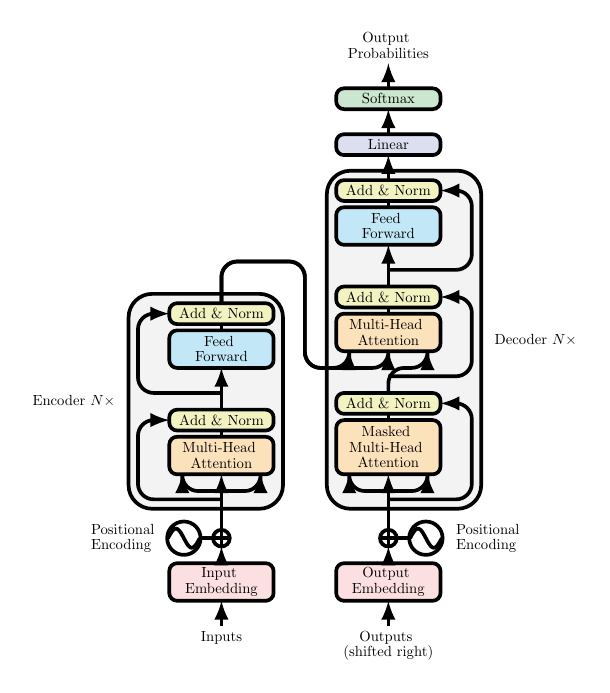
\begin{tikzpicture}[scale=0.53, every node/.style={scale=0.53}]
            \definecolor{emb_color}{RGB}{252,224,225}
            \definecolor{multi_head_attention_color}{RGB}{252,226,187}
            \definecolor{add_norm_color}{RGB}{242,243,193}
            \definecolor{ff_color}{RGB}{194,232,247}
            \definecolor{softmax_color}{RGB}{203,231,207}
            \definecolor{linear_color}{RGB}{220,223,240}
            \definecolor{gray_bbox_color}{RGB}{243,243,244}
            \draw[fill=gray_bbox_color, line width=0.046875cm, rounded corners=0.300000cm] (-0.975000, 6.455000) -- (2.725000, 6.455000) -- (2.725000, 1.305000) -- (-0.975000, 1.305000) -- cycle;
            \draw[fill=gray_bbox_color, line width=0.046875cm, rounded corners=0.300000cm] (3.775000, 9.405000) -- (7.475000, 9.405000) -- (7.475000, 1.305000) -- (3.775000, 1.305000) -- cycle;
            \draw[line width=0.046875cm, fill=emb_color, rounded corners=0.100000cm] (0.000000, 0.000000) -- (2.500000, 0.000000) -- (2.500000, -0.900000) -- (0.000000, -0.900000) -- cycle;
            \node[text width=2.500000cm, align=center] at (1.250000,-0.450000) {Input \vspace{-0.05cm} \linebreak Embedding};
            \draw[line width=0.046875cm, fill=emb_color, rounded corners=0.100000cm] (4.000000, 0.000000) -- (6.500000, 0.000000) -- (6.500000, -0.900000) -- (4.000000, -0.900000) -- cycle;
            \node[text width=2.500000cm, align=center] at (5.250000,-0.450000) {Output \vspace{-0.05cm} \linebreak Embedding};
            \draw[line width=0.046875cm, fill=add_norm_color, rounded corners=0.100000cm] (0.000000, 3.680000) -- (2.500000, 3.680000) -- (2.500000, 3.180000) -- (0.000000, 3.180000) -- cycle;
            \node[text width=2.500000cm, align=center] at (1.250000,3.430000) {Add \& Norm};
            \draw[line width=0.046875cm, fill=multi_head_attention_color, rounded corners=0.100000cm] (0.000000, 3.030000) -- (2.500000, 3.030000) -- (2.500000, 2.130000) -- (0.000000, 2.130000) -- cycle;
            \node[text width=2.500000cm, align=center] at (1.250000,2.580000) {Multi-Head \vspace{-0.05cm} \linebreak Attention};
            \draw[line width=0.046875cm] (1.250000, 3.030000) -- (1.250000, 3.180000);
            \draw[line width=0.046875cm, fill=add_norm_color, rounded corners=0.100000cm] (4.000000, 6.630000) -- (6.500000, 6.630000) -- (6.500000, 6.130000) -- (4.000000, 6.130000) -- cycle;
            \node[text width=2.500000cm, align=center] at (5.250000,6.380000) {Add \& Norm};
            \draw[line width=0.046875cm, fill=multi_head_attention_color, rounded corners=0.100000cm] (4.000000, 5.980000) -- (6.500000, 5.980000) -- (6.500000, 5.080000) -- (4.000000, 5.080000) -- cycle;
            \node[text width=2.500000cm, align=center] at (5.250000,5.530000) {Multi-Head \vspace{-0.05cm} \linebreak Attention};
            \draw[line width=0.046875cm] (5.250000, 5.980000) -- (5.250000, 6.130000);
            \draw[line width=0.046875cm, fill=add_norm_color, rounded corners=0.100000cm] (4.000000, 4.080000) -- (6.500000, 4.080000) -- (6.500000, 3.580000) -- (4.000000, 3.580000) -- cycle;
            \node[text width=2.500000cm, align=center] at (5.250000,3.830000) {Add \& Norm};
            \draw[line width=0.046875cm, fill=multi_head_attention_color, rounded corners=0.100000cm] (4.000000, 3.430000) -- (6.500000, 3.430000) -- (6.500000, 2.130000) -- (4.000000, 2.130000) -- cycle;
            \node[text width=2.500000cm, align=center] at (5.250000,2.780000) {Masked \vspace{-0.05cm} \linebreak Multi-Head \vspace{-0.05cm} \linebreak Attention};
            \draw[line width=0.046875cm] (5.250000, 3.430000) -- (5.250000, 3.580000);
            \draw[line width=0.046875cm, fill=add_norm_color, rounded corners=0.100000cm] (0.000000, 6.230000) -- (2.500000, 6.230000) -- (2.500000, 5.730000) -- (0.000000, 5.730000) -- cycle;
            \node[text width=2.500000cm, align=center] at (1.250000,5.980000) {Add \& Norm};
            \draw[line width=0.046875cm, fill=ff_color, rounded corners=0.100000cm] (0.000000, 5.580000) -- (2.500000, 5.580000) -- (2.500000, 4.680000) -- (0.000000, 4.680000) -- cycle;
            \node[text width=2.500000cm, align=center] at (1.250000,5.130000) {Feed \vspace{-0.05cm} \linebreak Forward};
            \draw[line width=0.046875cm] (1.250000, 5.580000) -- (1.250000, 5.730000);
            \draw[line width=0.046875cm, fill=add_norm_color, rounded corners=0.100000cm] (4.000000, 9.180000) -- (6.500000, 9.180000) -- (6.500000, 8.680000) -- (4.000000, 8.680000) -- cycle;
            \node[text width=2.500000cm, align=center] at (5.250000,8.930000) {Add \& Norm};
            \draw[line width=0.046875cm, fill=ff_color, rounded corners=0.100000cm] (4.000000, 8.530000) -- (6.500000, 8.530000) -- (6.500000, 7.630000) -- (4.000000, 7.630000) -- cycle;
            \node[text width=2.500000cm, align=center] at (5.250000,8.080000) {Feed \vspace{-0.05cm} \linebreak Forward};
            \draw[line width=0.046875cm] (5.250000, 8.530000) -- (5.250000, 8.680000);
            \draw[line width=0.046875cm, fill=linear_color, rounded corners=0.100000cm] (4.000000, 10.280000) -- (6.500000, 10.280000) -- (6.500000, 9.780000) -- (4.000000, 9.780000) -- cycle;
            \node[text width=2.500000cm, align=center] at (5.250000,10.030000) {Linear};
            \draw[line width=0.046875cm, fill=softmax_color, rounded corners=0.100000cm] (4.000000, 11.380000) -- (6.500000, 11.380000) -- (6.500000, 10.880000) -- (4.000000, 10.880000) -- cycle;
            \node[text width=2.500000cm, align=center] at (5.250000,11.130000) {Softmax};
            \draw[line width=0.046875cm] (1.250000, 0.600000) circle (0.200000);
            \draw[line width=0.046875cm] (1.410000, 0.600000) -- (1.090000, 0.600000);
            \draw[line width=0.046875cm] (1.250000, 0.760000) -- (1.250000, 0.440000);
            \draw[line width=0.046875cm] (5.250000, 0.600000) circle (0.200000);
            \draw[line width=0.046875cm] (5.410000, 0.600000) -- (5.090000, 0.600000);
            \draw[line width=0.046875cm] (5.250000, 0.760000) -- (5.250000, 0.440000);
            \draw[line width=0.046875cm] (0.350000, 0.600000) circle (0.400000);
            \draw[line width=0.046875cm] (-0.030000, 0.600000) -- (-0.014490, 0.629156) -- (0.001020, 0.657833) -- (0.016531, 0.685561) -- (0.032041, 0.711884) -- (0.047551, 0.736369) -- (0.063061, 0.758616) -- (0.078571, 0.778258) -- (0.094082, 0.794973) -- (0.109592, 0.808486) -- (0.125102, 0.818576) -- (0.140612, 0.825077) -- (0.156122, 0.827883) -- (0.171633, 0.826946) -- (0.187143, 0.822284) -- (0.202653, 0.813971) -- (0.218163, 0.802145) -- (0.233673, 0.786999) -- (0.249184, 0.768783) -- (0.264694, 0.747796) -- (0.280204, 0.724382) -- (0.295714, 0.698925) -- (0.311224, 0.671845) -- (0.326735, 0.643584) -- (0.342245, 0.614608) -- (0.357755, 0.585392) -- (0.373265, 0.556416) -- (0.388776, 0.528155) -- (0.404286, 0.501075) -- (0.419796, 0.475618) -- (0.435306, 0.452204) -- (0.450816, 0.431217) -- (0.466327, 0.413001) -- (0.481837, 0.397855) -- (0.497347, 0.386029) -- (0.512857, 0.377716) -- (0.528367, 0.373054) -- (0.543878, 0.372117) -- (0.559388, 0.374923) -- (0.574898, 0.381424) -- (0.590408, 0.391514) -- (0.605918, 0.405027) -- (0.621429, 0.421742) -- (0.636939, 0.441384) -- (0.652449, 0.463631) -- (0.667959, 0.488116) -- (0.683469, 0.514439) -- (0.698980, 0.542167) -- (0.714490, 0.570844) -- (0.730000, 0.600000);
            \draw[line width=0.046875cm] (6.150000, 0.600000) circle (0.400000);
            \draw[line width=0.046875cm] (5.770000, 0.600000) -- (5.785510, 0.629156) -- (5.801020, 0.657833) -- (5.816531, 0.685561) -- (5.832041, 0.711884) -- (5.847551, 0.736369) -- (5.863061, 0.758616) -- (5.878571, 0.778258) -- (5.894082, 0.794973) -- (5.909592, 0.808486) -- (5.925102, 0.818576) -- (5.940612, 0.825077) -- (5.956122, 0.827883) -- (5.971633, 0.826946) -- (5.987143, 0.822284) -- (6.002653, 0.813971) -- (6.018163, 0.802145) -- (6.033673, 0.786999) -- (6.049184, 0.768783) -- (6.064694, 0.747796) -- (6.080204, 0.724382) -- (6.095714, 0.698925) -- (6.111224, 0.671845) -- (6.126735, 0.643584) -- (6.142245, 0.614608) -- (6.157755, 0.585392) -- (6.173265, 0.556416) -- (6.188776, 0.528155) -- (6.204286, 0.501075) -- (6.219796, 0.475618) -- (6.235306, 0.452204) -- (6.250816, 0.431217) -- (6.266327, 0.413001) -- (6.281837, 0.397855) -- (6.297347, 0.386029) -- (6.312857, 0.377716) -- (6.328367, 0.373054) -- (6.343878, 0.372117) -- (6.359388, 0.374923) -- (6.374898, 0.381424) -- (6.390408, 0.391514) -- (6.405918, 0.405027) -- (6.421429, 0.421742) -- (6.436939, 0.441384) -- (6.452449, 0.463631) -- (6.467959, 0.488116) -- (6.483469, 0.514439) -- (6.498980, 0.542167) -- (6.514490, 0.570844) -- (6.530000, 0.600000);
            \draw[line width=0.046875cm, -latex] (1.250000, 3.680000) -- (1.250000, 4.680000);
            \draw[line width=0.046875cm, -latex] (5.250000, 6.630000) -- (5.250000, 7.630000);
            \draw[line width=0.046875cm, -latex] (5.250000, 9.180000) -- (5.250000, 9.780000);
            \draw[line width=0.046875cm, -latex] (5.250000, 10.280000) -- (5.250000, 10.880000);
            \draw[line width=0.046875cm, -latex] (1.250000, 0.000000) -- (1.250000, 0.400000);
            \draw[line width=0.046875cm, -latex] (1.250000, 0.800000) -- (1.250000, 2.130000);
            \draw[line width=0.046875cm, -latex] (5.250000, 0.800000) -- (5.250000, 2.130000);
            \draw[line width=0.046875cm, -latex] (5.250000, 0.000000) -- (5.250000, 0.400000);
            \draw[line width=0.046875cm] (0.750000, 0.600000) -- (1.050000, 0.600000);
            \draw[line width=0.046875cm] (5.450000, 0.600000) -- (5.750000, 0.600000);
            \draw[-latex, line width=0.046875cm, rounded corners=0.200000cm] (1.250000, 4.080000) -- (-0.750000, 4.080000) -- (-0.750000, 5.980000) -- (0.000000, 5.980000);
            \draw[-latex, line width=0.046875cm, rounded corners=0.200000cm] (1.250000, 1.530000) -- (-0.750000, 1.530000) -- (-0.750000, 3.430000) -- (0.000000, 3.430000);
            \draw[-latex, line width=0.046875cm, rounded corners=0.200000cm] (5.250000, 1.530000) -- (7.250000, 1.530000) -- (7.250000, 3.830000) -- (6.500000, 3.830000);
            \draw[-latex, line width=0.046875cm, rounded corners=0.200000cm] (5.250000, 4.480000) -- (7.250000, 4.480000) -- (7.250000, 6.380000) -- (6.500000, 6.380000);
            \draw[-latex, line width=0.046875cm, rounded corners=0.200000cm] (5.250000, 7.030000) -- (7.250000, 7.030000) -- (7.250000, 8.930000) -- (6.500000, 8.930000);
            \draw[-latex, line width=0.046875cm, rounded corners=0.200000cm] (1.250000, 1.730000) -- (0.312500, 1.730000) -- (0.312500, 2.130000);
            \draw[-latex, line width=0.046875cm, rounded corners=0.200000cm] (1.250000, 1.730000) -- (2.187500, 1.730000) -- (2.187500, 2.130000);
            \draw[-latex, line width=0.046875cm, rounded corners=0.200000cm] (5.250000, 1.730000) -- (4.312500, 1.730000) -- (4.312500, 2.130000);
            \draw[-latex, line width=0.046875cm, rounded corners=0.200000cm] (5.250000, 1.730000) -- (6.187500, 1.730000) -- (6.187500, 2.130000);
            \draw[-latex, line width=0.046875cm, rounded corners=0.200000cm] (1.250000, 6.230000) -- (1.250000, 7.230000) -- (3.250000, 7.230000) -- (3.250000, 4.680000) -- (4.312500, 4.680000) -- (4.312500, 5.080000);
            \draw[-latex, line width=0.046875cm, rounded corners=0.200000cm] (1.250000, 6.230000) -- (1.250000, 7.230000) -- (3.250000, 7.230000) -- (3.250000, 4.680000) -- (5.250000, 4.680000) -- (5.250000, 5.080000);
            \draw[-latex, line width=0.046875cm, rounded corners=0.200000cm] (5.250000, 4.080000) -- (5.250000, 4.680000) -- (6.187500, 4.680000) -- (6.187500, 5.080000);
            \draw[line width=0.046875cm, -latex] (1.250000, -1.500000) -- (1.250000, -0.900000);
            \draw[line width=0.046875cm, -latex] (5.250000, -1.500000) -- (5.250000, -0.900000);
            \draw[line width=0.046875cm, -latex] (5.250000, 11.380000) -- (5.250000, 11.980000);
            \node[text width=2.500000cm, anchor=north, align=center] at (1.250000,-1.500000) {Inputs};
            \node[text width=2.500000cm, anchor=north, align=center] at (5.250000,-1.500000) {Outputs \vspace{-0.05cm} \linebreak (shifted right)};
            \node[text width=2.500000cm, anchor=south, align=center] at (5.250000,11.980000) {Output \vspace{-0.05cm} \linebreak Probabilities};
            \node[anchor=east] at (-1.175000,3.880000) {Encoder $N\times$};
            \node[anchor=west] at (7.675000,5.355000) {Decoder $N\times$};
            \node[text width=2.000000cm, anchor=east] at (0.250000,0.600000) {Positional \vspace{-0.05cm} \linebreak Encoding};
            \node[text width=2.000000cm, anchor=west] at (6.750000,0.600000) {Positional \vspace{-0.05cm} \linebreak Encoding};
        \end{tikzpicture}
    \end{center}

\end{frame}

\begin{frame}[fragile]{Attention (Self-Attention Mechanism)}

    \begin{itemize}
        \item Assume we want to translate a sentence: ”The animal didn't cross the street because it was too tired”
    \end{itemize}
    \begin{center}
        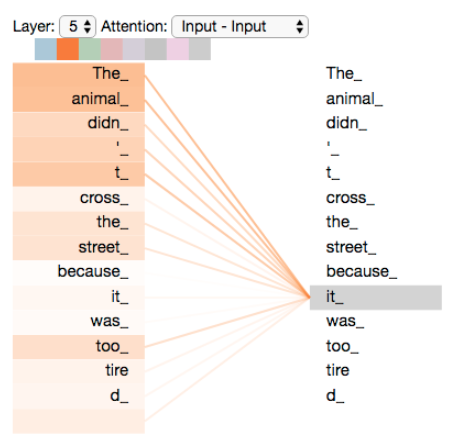
\includegraphics[scale=0.25]{../images/img_7.png} \\
        \href{https://jalammar.github.io/illustrated-transformer/}{[Image Source]}
    \end{center}
    \begin{itemize}
        \item Advantages:
              \begin{enumerate}
                  \item Interaction distance
                  \item Parallelizability
                  \item Interpretability
              \end{enumerate}
    \end{itemize}

\end{frame}

\begin{frame}[fragile]{Masked Self-Attention}

    \begin{itemize}
        \item Masked Self-Attention prevents a word to peak at tokens to its right.
    \end{itemize}

    \begin{center}
        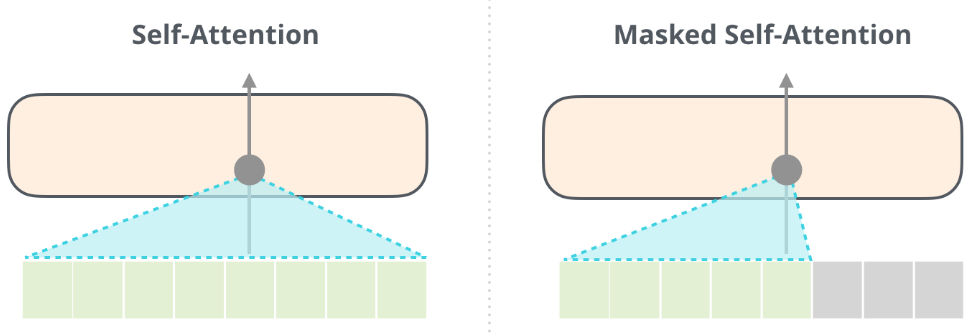
\includegraphics[scale=0.3]{../images/img_11.png} \\
        \href{https://jalammar.github.io/illustrated-gpt2/}{[Image Source]}
    \end{center}

    \begin{itemize}
        \item This distinction is the major difference between GPT and BERT.
    \end{itemize}

\end{frame}